\section*{Part B}
\addcontentsline{toc}{section}{Part B}

\begin{tcolorbox}
  B.1) Write $f(t)$ in Fourier synthesis form.
\end{tcolorbox}

\[ f(t)= \sum_{n=1}^{\infty} \frac{2V}{\pi n}\sin2\pi n f_o t \]

\begin{tcolorbox}
  B.2) Calculate the first 10 sinewave coefficients.
\end{tcolorbox}

\lstinputlisting[
  caption = Requirement 2 MATLAB code,
  label = code:B_r_2,
]{matlab/B_r_2.m}

\[ b[n]\Big\rvert_{n=1}^{10} = {\frac{2V}{\pi}, \frac{V}{\pi}, \frac{2V}{3\pi}, \frac{V}{2\pi}, \frac{2V}{5\pi}, \frac{V}{3\pi}, \frac{2V}{7\pi}, \frac{V}{4\pi}, \frac{2V}{9\pi}, \frac{V}{5\pi}} \]

\begin{tcolorbox}
  B.3) Synthesise the first 10 harmonics of this waveform and plot the result.
\end{tcolorbox}

\lstinputlisting[
  caption = Requirement 3 and Question 1 and 2 MATLAB code,
  label = code:B_r3_and_q,
]{matlab/B_r3_and_q.m}

\begin{figure}[htbp]
  \centering
  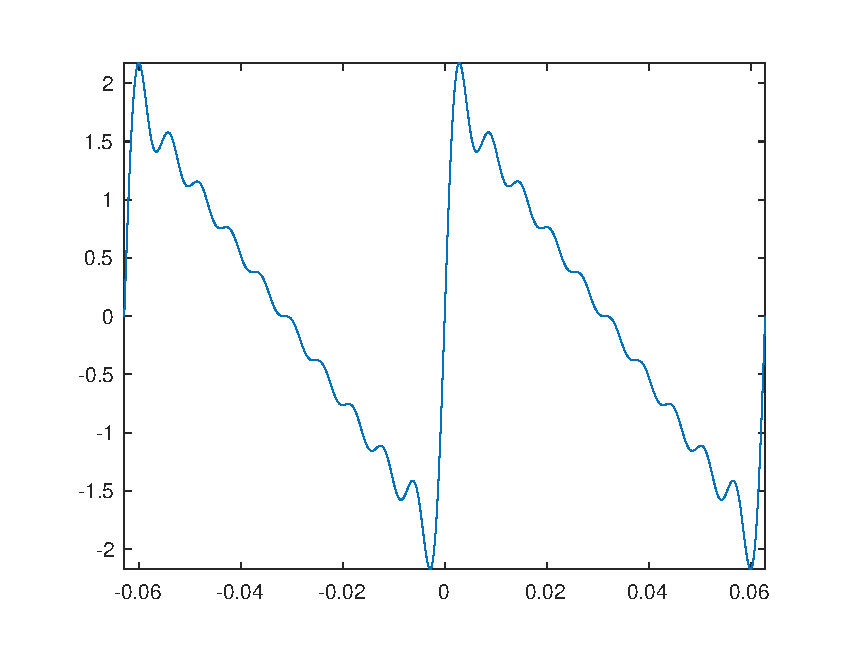
\includegraphics[width=2.8in]{matlab/fig/B_r_3.eps}
  \caption{the first 10 harmonics of the sawtooth waveform}    
  \label{fig:B_r_3}
\end{figure}

\pagebreak

\begin{tcolorbox}
  B.4) Plot in the same figure the original and synthesised sawtooth waveforms. Compare the resulting waveform with what you expected to see and discuss the results.
\end{tcolorbox}

\begin{figure}[h]
  \centering
  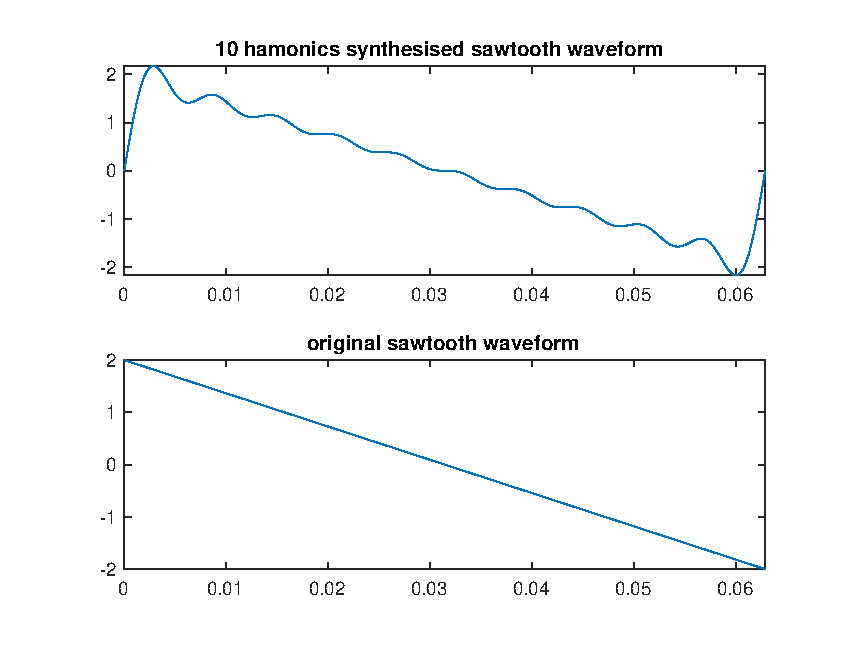
\includegraphics[width=3in]{matlab/fig/B_q_1.eps}
  \caption{10 harmonics synthesised sawtooth waveform with its origin}    
  \label{fig:B_q_1}
\end{figure}

The desired result is a vertical straight line at both ends and a diagonal straight line in the middle. 10 harmonics synthesised signal has slightly sloping ends and an undulating overshoot in the middle.

\begin{tcolorbox}
  B.5) If the number of harmonics is reduced to 5, comment on the changes that will be observed practically.
\end{tcolorbox}

\begin{figure}[h]
  \centering
  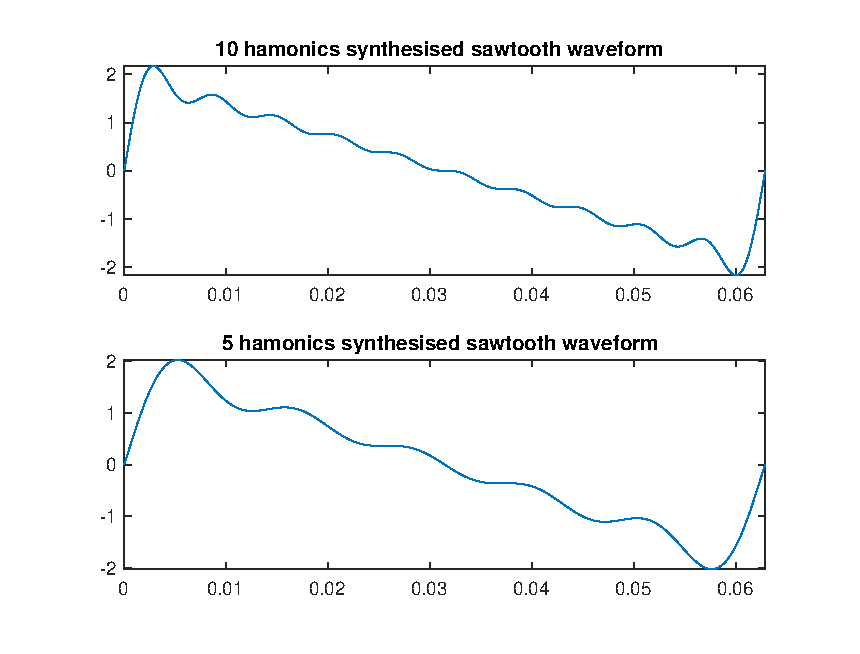
\includegraphics[width=3in]{matlab/fig/B_q_2.eps}
  \caption{10 harmonics synthesised with 5 harmonics synthesised sawtooth waveform}    
  \label{fig:B_q_2}
\end{figure}

The less harmonics used, the higher the deviation from the original signal.

\pagebreak